\chapter{General Introduction}
\label{chap:introduction}


\begin{figure}[h]
  \centering
  \includegraphics[width=.55\textwidth]{ch1-introduction/snake_complexity.pdf}
\end{figure}

\begin{quoteshrink}
  ``It is interesting to contemplate a tangled bank...''

\hfill{Charles Darwin}
\end{quoteshrink}


\noindent
The ability to both obtain and avoid becoming food is one of the primary selection pressures driving animal evolution. Predator-prey interactions not only shape the species directly involved, but also form the fundamental building blocks of ecosystem structure, making them key to our understanding of biological systems as a whole \citep{pimm1984complexity,cohen1990community}. While these interactions are ubiquitous across diverse environments and ecosystems, each predator-prey interaction plays out within its own specific context. For example, two predators may rely on two different strategies to capture the same prey, such as relying on venom or manoeuvrability, despite being similar in size and form. However, amongst these context dependencies, certain patterns emerge that provide a clear approach to understand how these interactions emerge and affect the systems in which they are embedded.


While the arms race between predators and their prey plays out across a diversity of forms, all players must abide to the fundamental constraints imposed by physics. For example biomechanical and physiological limitations result in flying species remaining relatively small \citep{chatterjee2007aerodynamics,dudley2002mechanisms} while the largest species are invariably found in the oceans due to buoyancy \citep{heim2015cope}. It is within these boundaries of physics that evolution trades off between the benefits of investing in traits relating to predator-prey interactions and the energetic costs associated with developing such traits. One common way for these trades-offs to present themselves is through their link with both body size and the dimensionality of these interactions (Figure 1.).
%need to write up this figure caption.

Since Kleiber fist demonstrated the link between the rate of energy utilised by an animal and its size \citep{kleiber1947body}, ecologists have utilised this correlation to understand a range of biological processes and principles \citep{sibly2012metabolic,west1997general,brown2004}. More recent formulations have attempted to use the fractal structure of physiological systems as a first principle approach to unify many aspect of biology including physiology, behaviour and ecology \citep{west1997general,brown2004}. Despite the heated debate surrounding the exact nature of this scaling and the fundamental basis that underpins it \citep{isaac2010metabolic}, this scaling relationship has become one of the most useful proxies to many elements of biology, including predator-prey interactions \citep{brown2004}. While body size and metabolic rate have featured as the main focus of this drive to find fundamental elements within biological complexity the dimensionality of the arena these interactions play out in has more recently gained attention as a key component.


Similar to the formalisation of metabolic theory in the mid 90s, the role of habitat complexity in biology has its roots in utilising the mathematics of fractals in order to explain macroecological patterns. \cite{morse1985fractal} were the first to use this geometry to describe how the space filling properties of vegetation can determine arthropod community densities through habitat availability. This approach of defining dimensionality using fractals has been used to determine the effects of dimensionality across numerous ecological systems \citep{kenkel1996fractals,shorrocks1991fractal,gunnarsson1992fractal,gee1994body,jeffries1993invertebrate} and used as a general approach to define ecological structure \citep{cohen1995marine,henderson2010linking}. More recently however, the focus of dimensionality has shifted from that of the habitat to that of the interactions themselves.


\begin{figure}[!Hpt]
  \centering
  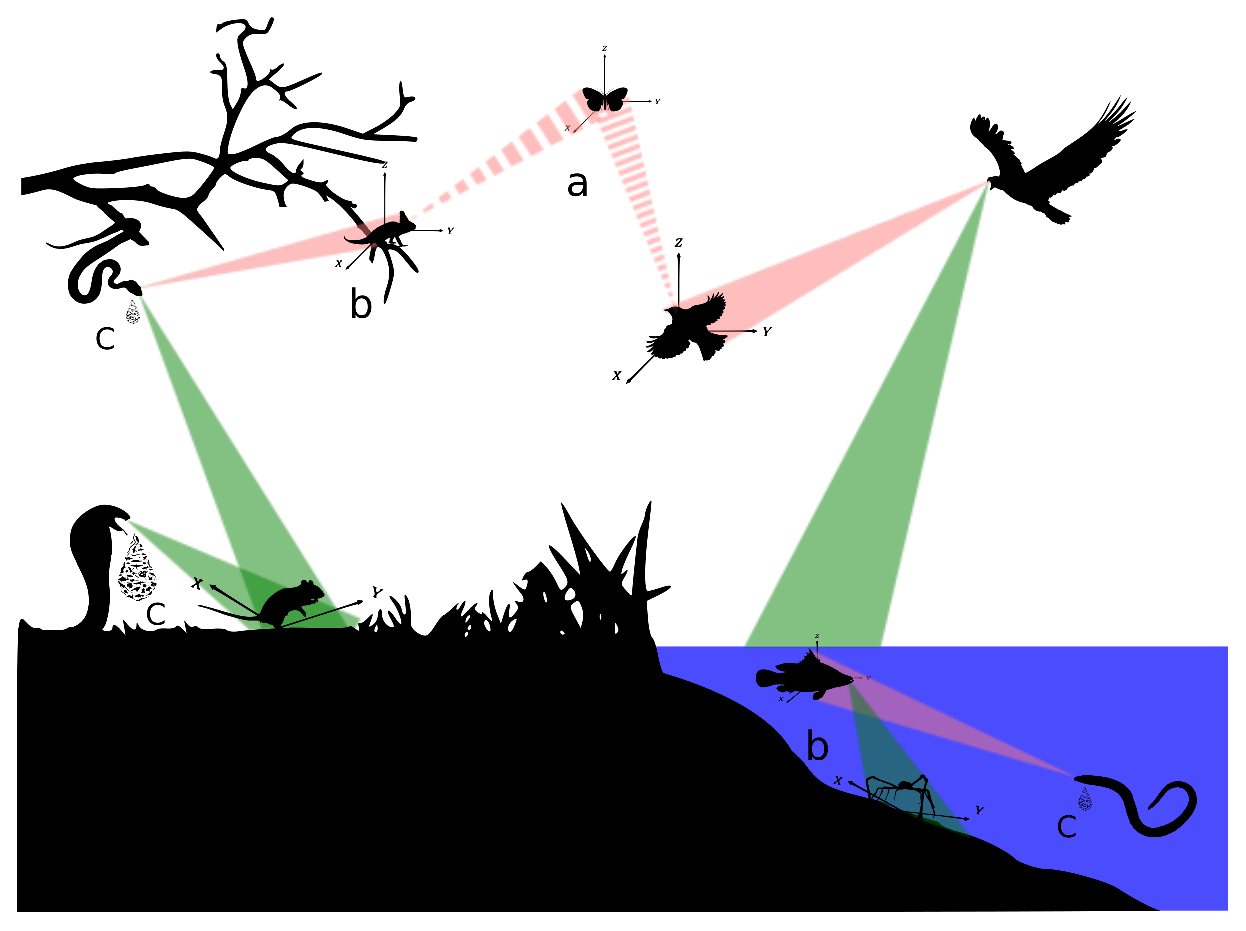
\includegraphics[keepaspectratio=true, width=1.0\textwidth,left]{ch1-introduction/fig_into.eps}\hspace*{10cm}
  \caption[ ]{If a species searches across a habitat surface, such as a terrestrial or water surface, the interaction can be defined as 2D (Green cones). If a species searches across a volume, such as pelagic or aerial environments, the interaction can be defined as 3D (Red cones). As arboreal habitats display the space filling properties of an object with a dimensionality higher than a two dimensional object, searching such volumes would also constitute high dimensional interactions. The dimensionality of the environment a species resides within is also likely to influence its ability to escape. Species in high dimensional habitats, such as pelagic, arboreal and aerial environments, have more routes of escape in comparison to species in low dimensional habitats such as terrestrial and benthic habitats. Interactions are also dependent on the ability of species to sample the temporal dimension with high temporal resolution allowing for more accurate tracking of predator or prey movements. This thesis explores several factors associated with interaction dimensionality including; a. The link between temporal perception, body size and metabolic rate; b. How escape space may affect life-history evolution; c. how the dimensionality of the habitat may affect predator traits evolution, in particular venom.}
  \label{fig:Figure 1.1}
\end{figure}


While species may be associated with habitats of different dimensions, for example the two dimensions of terrestrial systems or the three dimensions of open pelagic systems, the interaction dimensionality mainly depends on where the prey species resides. For example, a bird may be within a 3D aerial environment while flying, but is effectively foraging over a 2D habitat (Figure 1). Such a bird would hence experience the foraging limitations of two dimensional space but also the predation pressures and escape strategies associated with existing within three dimensions \citep{pawar2012dimensionality}. This framework allows dimensionality to be explored across groups and foraging strategies and extends the predictive ability of body mass scaling through incorporating the difference in the scaling of interaction rates across interaction dimensionality. 
It also opens up the importance of the role of sensory ecology within such interactions, in particular as such sensory systems may show different scaling in comparison to that predicted from metabolic theory \citep{mcgill2006allometric,kiltie2000scaling}. 
%is that last sentance kinda setting you up for a bit of a fall? is the scaling in kiltie predicted from metabolic theory? see  Howard C Howland, , Stacey Merola, Jennifer R Basarab which has a scaling of 0.2 between vidual accuity and size.


This thesis draws on how both body size and dimensionality, two aspects that intersect physics and biology, affect predator-prey interactions across the range of contexts these predator-prey interactions take place. By using comparative methods I will focus on three areas; how do species sample and perceive the temporal dimension; the role of habitat dimensionality in prey species life history; and the role of habitat dimensionality in the evolution of predatory traits. By understanding the forces shaping species within the dimensions of their habitats we can gain deeper understanding of the mechanics of predator-prey interactions as a whole.\\


\section{\uppercase{R}esearch outline}


\textbf{Chapter 2: Body size, metabolic rate and visual temporal perception in vertebrates.}


 All organisms must perceive the temporal dimension of their environment. This is particularly true of predators and their prey that need to accurately track and predict their adversaries' motion. Here I collate data on a measure of visual temporal perception called critical flicker fusion to test whether species that are predicted to be more maneuverable or more physiologically capable to process temporal information can perceive events at finer scales. I show that, as expected, small species with high metabolic rates have the fastest perception of time. This has important consequences for the ability of predators to capture their prey and I discuss some examples of adaptations in predator species that potentially mitigate against the need for small size and a high metabolic rate.\\


\textbf{Chapter 3: Ecology and mode-of-life explain lifespan variation in birds and mammals.}


Maximum lifespan varies strongly with body mass yet many species live far longer than expected given their size. This may reflect interspecific variation in extrinsic mortality, as life-history theory predicts investment in long-term survival when extrinsic mortality is reduced. Here, I investigate how ecological and mode-of-life traits that are predicted to reduce extrinsic mortality influence lifespan across mammals and birds. I show that species associated with high dimensional habitats, namely arboreal and volant species, show longer lifespan than expected for their body size. I discuss how habitat dimensionality may affect exposure of prey to predation pressures and the role of other ecological traits including fossoriality, eusociality, and activity patterns.\\




\textbf{Chapter 4: Habitat dimensionality and a diet of eggs; the evolution of venom loss in snakes.}


Despite the obvious advantages of possessing venom there is little explanation for variation in the volume and toxicity of venom in snakes. This is particularly apparent in species that partially or fully lose the capacity to produce venom such as demonstrated in sea snake species. As venom is primarily used for capturing prey I test whether fundamental factors, including habitat dimensionality and diet, affect the amount of venom produced within a species through their influence of encounter rates and prey toxicity resistance. By collating data on venom toxicity (LD$_{50}$), diets, body size, environment dimensionality and both maximum and minimum venom volumes comprising of 101 species, I show that species found in high dimensional environments or that have egg-based diets produce less venom than their counterparts. I also demonstrate the general prey-specific nature of venom toxicity using phylogenetic distance between diet species and LD$_{50}$ model species as a test. I discuss the possible mechanisms and the implications of these results in relation to both the evolution of venom and costly predatory traits in general.\\

%
%
Finally, in \textbf{Chapter 5}, I close with a discussion of the importance of including dimensionality in macroecological models and the future methodologies and directions relating to the research presented in this thesis.


\section{\uppercase{A}dditional work}
In addition to the chapters enclosed in this thesis, I have also been involved in the following research during my studies:\\

\begin{singlespace}
Donohue, I., Petchey, O.L., Montoya, J.M., Jackson, A.L., McNally, L., Viana, M., Healy, K., Lurgi, M., O\'Connor, N.E. \& Emmerson, M.C. (2013). On the dimensionality of ecological stability. Ecology Letters, 16(4), 421-429. \\
\end{singlespace}

\noindent
I was involved with the conception, data analysis and write-up of this paper. \\

\begin{singlespace}
Kane, A., Ruxton, G.D., Jackson, A.L. \& Healy, K.(2015). Body size drives importance of scavenging in theropods. Submitted to \textit{The American Naturalist}. \\
\end{singlespace}

\noindent
I was involved with the conception, data collection, analysis and write-up of this paper. \\



%\bibliographystyle{PLoS-Biology}
%\bibliography{bibfile}

